\documentclass[11pt,conference,a4paper,twocolumns,romanappendices]{IEEEtran}
\usepackage[utf8]{inputenc}
\usepackage[english]{babel}
\usepackage{verbatim}
\usepackage{graphicx}
\usepackage{wrapfig}
\author{Lucas Colantuono, Lucas Kummer, Shanan Lynch, Samuel Sedlmeir}

\title{IoT Trace Analysis}
\date{\today}
\markboth{Improving local transports by analysing taxi meta data}{}

\author{\IEEEauthorblockN{Lucas Colantuono}
\IEEEauthorblockA{INSA Lyon \\
lucas.colantuono@insa-lyon.fr}
\and
\IEEEauthorblockN{Lucas Kummer}
\IEEEauthorblockA{INSA Lyon\\
lucas.kummer@insa-lyon.fr}
\and
\IEEEauthorblockN{Shanan Lynch}
\IEEEauthorblockA{INSA Lyon\\
shanan.lynch@insa-lyon.fr}
\and
\IEEEauthorblockN{Samuel Sedlmeir}
\IEEEauthorblockA{INSA Lyon\\
S.Sedlmeir@campus.lmu.de}}

\begin{document}

\maketitle

\tableofcontents
\newpage

\begin{abstract}
 
\end{abstract}

\section{Introduction}
\label{sec:Introduction}

\section{Related work}
There are several different articles, that analyse the same or similar datasets and compute different models and metrics. \\
The first article written by chinese researchers analysed the Taxi GPS traces from Shanghai in order to develop a model that helps understanding the needs of vehicular ad hoc networks for example. Therefore the authors computed several metrics, e.g. the turn probability at all the road crossings, implemented a map-matching algorithm and considered macro- and microscopic travel patterns. Their so called "META" model shows a higher accuracy than all other models at this time. \cite{meta} \\
A different approach is presented by American researchers in their article. They haven't used GPS traces, but collected traces from users on a campus via WiFi routers, at which the users' smartphones automatically registered at. Thereby they are able to develop a model, which makes it possible for them to detect a hierarchy of the different access points and cluster them. These cluster are being analysed in terms of the size distribution as well as inter- and intra-cluster travel patterns. \cite{wlan} \\
Another article about the taxi data set from Shanghai aimed to find an algorithm, that allows fair route sharing for every competing taxi driver. One of its goals is to not lose efficiency and a driving cost per customer as low as possible, so that it offers advantages for the driver and the customer equally. This requires a complex evaluation algorithm that considers several priniciples which are respected by the assignment mechanism. \cite{scram} \\
In contrast to other public transports, taxi drivers plan their own routes once they drop off a passenger. Some articles are about recommender routes that aim to save the time of taxi drivers and potential passengers. \\
In general, there are three ways to develop recommender systems. The first one is content based which means suggesting items that are similar to those a given user liked in the past. The second way is based on recommendations computed according to the tastes of other users similar to the target user. The third one is an hybrid solution. \\
T-Finder provides taxi drivers with detailed information not only about the route, but also about parking places. \cite{tf} The goal of the work described in this article is to propose an approach to detect parking places based on a large number of GPS trajectories generated by taxis, where the parking places stand for the locations where taxi drivers usually wait for passengers with their taxis parked. T-Finder enhances the passenger recommender by estimating the waiting time on a specified nearby road segment in addition to calculating the probability of finding a vacant taxi. \\
LCP \cite{eff} uses the same method as T-Finder \cite{tf} to extract the representative small areas from the trajectories. The goal of the LCP route recommendation algorithm is to find an energy-efficient mobile recommender system by exploiting the energy-efficient driving patterns extracted from the location traces of Taxi drivers. This system has the ability to recommend a sequence of potential pick-up points for a driver in a way such that the potential travel distance before having customer is minimized. \\
Identifying user interests and providing personalized suggestions, the different recommender systems address and collect information to reduce the spent time of passengers and taxi drivers. Recommender systems \cite{tow} presents an overview of the field of recommender systems and describes the current generation of recommendation methods and various ways to extend the capabilities of recommender systems as well. This article concluded that recommender systems made significant progress over the last decade when numerous content-based, collaborative and hybrid methods were proposed and several "industrial-strength" systems have been developed. \\
Recommender systems by mining large-scale \cite{min1,min2} data develop a smart recommendation system based on extracted patterns and data from studies focused of large-scale trace data collected by a probe taxi. Large-scale trace data provide us with opportunities to extract useful transportation patterns and utilize these patterns to improve efficiency.
\section{Data consistency}
The first task is to check and improve the consistency of the provided data, so that we are able to compute our chosen metric accurately. \\
At the beginning we have to filter all impossible values of the variables we're operating on. For example, our R script removes all entries with a negative speed value or timestamps outside of the interval in which these data have been collected.  Apparently the trace files only contain consistent data sets as our script has not detected and removed a single error. \\
Furthermore, there are two more types of errors that have to be considered: Checking the geographical consistency and filtering gaps in the traces.
\subsection{Geographical consistency}

In the next step we analysed several statistical metrics concerning the speed variable which showed that there is a wide spectrum of different values, with some outliers bigger than 200 km/h, which does not make any sense in a city centre and is probably an error. That's why we decided to cut off all the entries with a speed higher than three times the interquartile range. As you can see in figure \ref{fig:speed_before} the speed distribution is skewed right with a single maximum. That justifies our decision, because we don't lose relevant data entries, when we choose our cut-off speed value. On the other hand side, just performing a coordinate cut is not sufficient: it changes the speed distribution slightly, e.g. we lost some data entries on the street towards one of the airports by removing all the points with a speed higher than 80 km/h. However, it does not remove all error entries. \\

\begin{figure}[h]
\centering
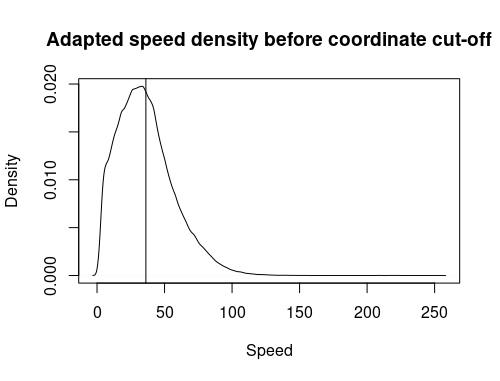
\includegraphics[scale=0.6]{density_before.png}
\caption{\label{fig:speed_before}Adapted speed distribution without zero values, but before coordinate filtering}
\end{figure}

The data has still to be filtered by the coordinates. As we decided to focus on the city centre, we only keep those entries in our dataset that have a longitude between 121.38 and 121.57 and a latitude between 31.15 and 31.32. In figure \ref{fig:borders} you can see our chosen borders on a map with a random sample of 100.000 points. \\

\begin{figure}[h]
\centering
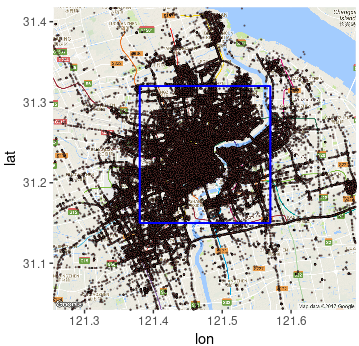
\includegraphics[scale=0.9]{borders.png}
\caption{\label{fig:borders}Borders of the city center}
\end{figure}

After restricting the data to this area, we observed a change in the distribution of the speed values as well: In general, the mean slightly decreases, in this case from 35.57 km/h to 33.46 km/h, whilst the median is increasing more significantly, as the amount of datasets with a speed higher than the median that we remove (in this case) comes up to more than 30 percent of all datasets. As we have a right skewed distribution, we eliminate higher values with this procedure, which is the result of the fact that some streets outside of the city center don't have a low speed limit and make it necessary to perform this cut-off: for example it decreases the amount of datasets with a speed higher than 80km/h by more than one half, see figure \ref{fig:speed_after}. \\

\begin{figure}[h]
\centering
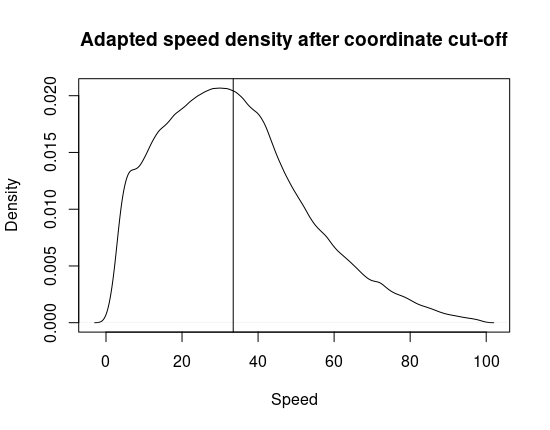
\includegraphics[scale=0.6]{density_after.png}
\caption{\label{fig:speed_after}Adapted speed distribution without zero values, after coordinate filtering}
\end{figure}

\subsection{Gap filtering}
After this procedure we are already able to plot a schematic map of Shanghai, although our dataset still contains data to be filtered. We search for those taxi traces with a time gap between two data entries. This gap could either be a result of a data transmission error or an indicator for the beginning of a new taxi trip.\\
\begin{figure}[h]
\centering
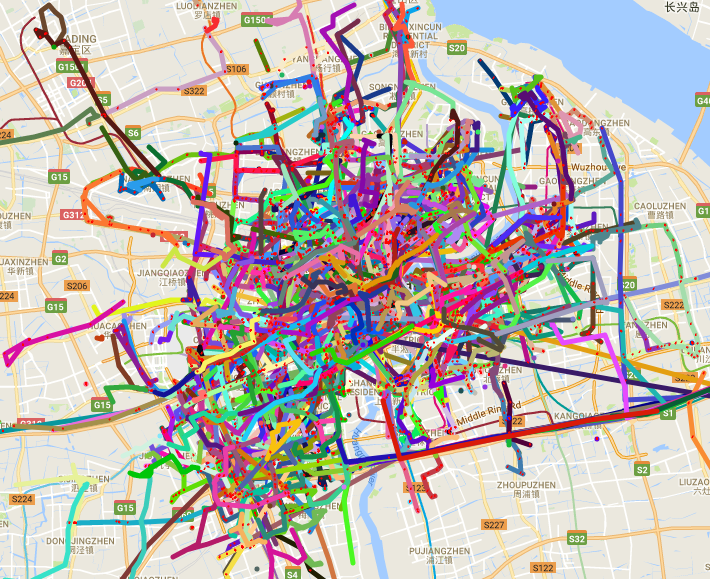
\includegraphics[scale=0.35]{plotalltrips.png}
\caption{\label{fig:plotalltrips}All calculated trips}
\end{figure}
To define these trips we had to choose a time gap that was appropriate for this data. So to define a trip we said that if the absolute value of a time gap between two data was bigger than 600 seconds that it would be separated and be a new trip.\\
As you can see in figure \ref{fig:timegap}, the mean value is around 25 minutes per gap in this case, while most of the gaps are shorter than 20 minutes. \\
\begin{figure}[h]
\centering
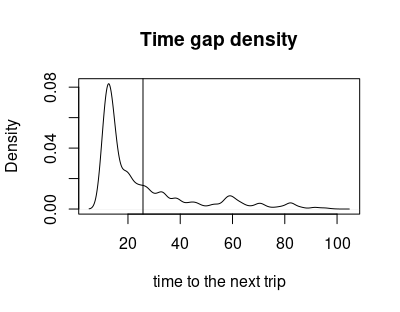
\includegraphics[scale=0.75]{timegap.png}
\caption{\label{fig:timegap}The time-gap distribution}
\end{figure}
The reason we chose this time range was so that for future analyses of these trips we felt that this time range would keep our results consistent and more accurate. Each of these trips would be given random colours to discern one from another if we decided to plot all of these trips like in the example given. As you can see there are many trips that have been plotted and to the eye these trips seem to be valid as well. \\

\section{Heatmaps}
The previously treated data can now be used to plot a row of heatmaps. Therefore we can vary several parameters in order to affect the appearance and its content. \\
\subsection{Appearance parameters}
As appearance parameters we can define the center position of the heatmap which will be positioned in the very center of Shanghai. Apart from that we can define the threshold, radius, gradient, opacity and a dissipating factor. The threshold is a value that defines how many datapoints are required at a certain spot in order to be displayed as a different coloured circle which size is defined by the radius. The gradient parameter controls the colour gradient, whereas the opacity variable is responsible for the degree of transparency the circles will show. The dissipating factor controls whether the data is scattering as soon as one zoomes into the map.
Amongst those parameters, we focus on the radius parameter, as it has the biggest influence. It highly depends on the size of the heatmap: the further we zoom is, the smaller the radius must become, otherwise we will display huge circles on a high-level-zoom map, which contain hardly any information.

\subsection{Content parameters}
Even more important than the appearance parameters are the parameters of the data to be displayed.
As we cannot display all available data points, we take a random sample of a big data file, in order to get an equally distributed selection of times and taxis. Observations have shown, that this sampling gets very close to using ways more data.
After sampling we can make use of different parameters to either plot all data or just those with or without a passenger.
A splitting of all available data into several time slots is useful as well - in order to observe different patterns or preferred quarters of the taxis.
As you can see in figure \ref{fig:h3to6} and \ref{fig:h15to18} it is simply visible: Between 3 and 6 a.m. there is a high density in the northern center, whereas between 3 and 6 p.m. the taxis a more concentrated in the very center of Shanghai and not that strongly scattered all over the map.

\begin{figure}[h]
\centering
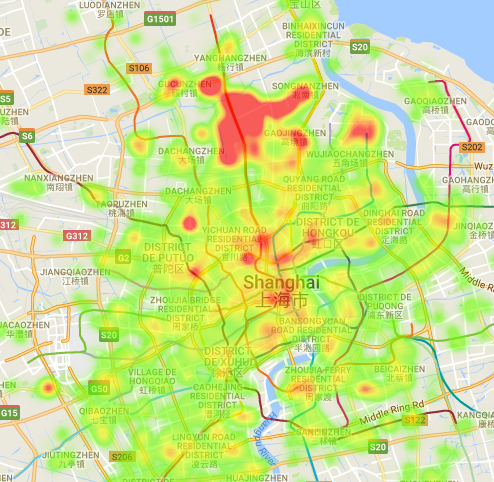
\includegraphics[scale=0.45]{3to6.png}
\caption{\label{fig:h3to6}Heatmap of all taxis between 3 and 6 a.m.}
\end{figure}

\begin{figure}[h]
\centering
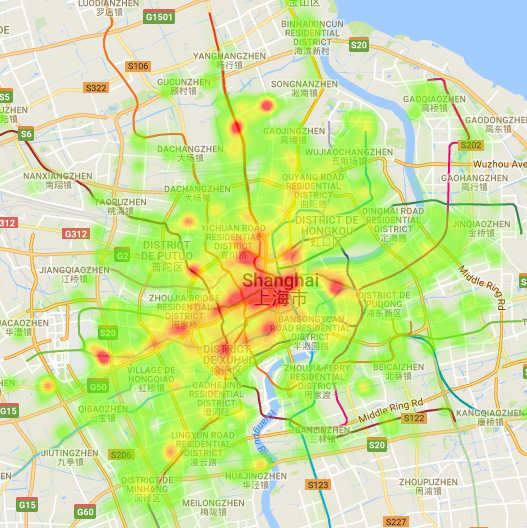
\includegraphics[scale=0.45]{15to18.png}
\caption{\label{fig:h15to18}Heatmap of all taxis between 3 and 6 p.m.}
\end{figure}


\section{Future work}

In order to customize and create heat maps more easier, future work will need to create an interface where data can filtered by criteria like if the taxi has or not passengers, taxiID, date, speeds, position and hours. Also split into different range hours heatmaps, in this case could be possible to use the code developed and described on this paper to create heatmaps, asking by ui the range hour. \\
We can plan to deploy our work with real data in the future to detect the places that are collapsed and we can suggest something to improve the traffic. Taking into consideration these cases, we will validate the effectiveness of the system. \\
Furthermore, future work will need to define some rules to detect 'friendly' taxis. For example, by work's hours and proximitely. In order to do that, we can scale our heatmap's code by defining a short distance when taxis are without passenger and in the same time. After that, we will get the taxis that are connected by these rules.

\section{Summary}

\newpage
\bibliography{biblio}
\bibliographystyle{IEEEtran}

\end{document}
